\documentclass{report}
\usepackage{graphicx} % Required for inserting images
\usepackage{booktabs} % For better horizontal lines
\usepackage{tabularx} % For width-adjustable tables
\usepackage{amsmath} % Math typesetting
\usepackage{gensymb} % Degree symbol
\usepackage{float} % To force table placement
\usepackage{setspace}    % To adjust line spacing

\begin{document}

\begin{titlepage}
    \centering

    \setstretch{1.5}
    {\Large \textbf{MACHINE LEARNING MODELS FOR PREDICTIVE ANALYSIS OF PRESSURE DROP AND TEMPERATURE IN POLYMER ELECTROLYTE MEMBRANE FUEL CELL STACKS TO FIND OPTIMAL FABRICATION PARAMETERS}}
    
    \vspace{5em}
    
    {\Large \textbf{HANHEE LEE}}
    
    \vfill
    
    {\Large ESROP GLOBAL}
    
    \vspace{1em} {\Large NATIONAL UNIVERSITY OF SINGAPORE}
    
    \vspace{1em} {\Large 2024}
    
\end{titlepage}

\pagenumbering{roman}

\begin{center}
    \section*{Declaration}
    I hereby declare that the thesis is my original work and it has been written by 
    me in its entirety. I have duly acknowledged all the sources of information 
    which have been used in this thesis. 
    
    \vspace{1em} \noindent This thesis has also not been submitted for any degree in any university previously 
    
    \vspace{1em} \noindent Hanhee Lee
    
    \vspace{1em} \noindent August, 2024
\end{center} 

\begin{center}
    \newpage \section*{Acknowledgements}
\end{center}
    \noindent I would like to express my sincere gratitude to Professor Erik Birgersson. Professor Birgersson has provided me with profound insights and knowledge on various topics, including polymer electrolyte membrane fuel cell stacks, machine learning, deep learning, and the use of COMSOL. He has also taught me how to effectively present to a scientific audience and the importance of learning independently. His enthusiasm and encouragement have made this journey a truly pleasant and enriching experience.

\begin{center}
    \newpage \section*{Abstract}    
\end{center}

\newpage \tableofcontents

\newpage \listoffigures

\newpage \listoftables

\newpage \section{List of Symbols}

    % Define custom column types with different proportional widths
    \newcolumntype{A}{>{\hsize=0.5\hsize}X} % Adjust these ratios as needed
    \newcolumntype{B}{>{\hsize=1.5\hsize}X}
    \newcolumntype{C}{>{\hsize=0.5\hsize}X}

    % Variables Table
    \begin{table}[h]
    \centering
    \begin{tabularx}{\textwidth}{ABC}
    \toprule
    \textbf{Name} & \textbf{Description} & \textbf{Unit} \\ 
    \midrule
    \( p \) & Pressure & Pa \\ 
    \( \mathbf{u}, \mathbf{U} \) & Velocity & m/s \\ 
    \( \rho \) & Density & kg/m$^3$ \\ 
    \( \mathbf{I} \) & Identity tensor & - \\ 
    \( \mathbf{K} \) & Viscous stress tensor & - \\ 
    \( \mathbf{F} \) & Volume force vector & - \\ 
    \( \mu \) & Dynamic viscosity & Pa$\cdot$s \\ 
    \( T \) & Temperature & K \\ 
    \( \mathbf{n} \) & Unit vector normal to the given surface & - \\ 
    \( \mathbf{G} \) & Reciprocal wall distance & - \\ 
    \( C_p \) & Specific heat capacity & J/(kg$\cdot$K) \\ 
    \( \mathbf{q} \) & Heat flux vector & - \\ 
    \( Q \) & Heat source & W/m$^3$ \\ 
    \( k \) & Thermal conductivity & W/(m$\cdot$K) \\ 
    \( R \) & Thermal resistance & (m$^2$$\cdot$K)/W \\ 
    \( d \) & Thin layer thickness & m \\ 
    \( \Delta \) & Delta & - \\ 
    \( \ell \) & Length/Distance & m \\ 
    \( u^+ \) & Tangential velocity in viscous units & - \\ 
    \( \sigma_w \) & Smoothing parameter & - \\ 
    Re & Reynolds number & - \\ 
    \( q \) & Quadratic loss coefficient & - \\ 
    \( \epsilon_p \) & Porosity & - \\ 
    \( \kappa \) & Permeability & m$^2$ \\ 
    \( \beta_F \) & Forchheimer coefficient & kg/m$^4$ \\ 
    \( Q_m \) & Mass source & kg/(m$^3$$\cdot$s) \\ 
    \bottomrule
    \end{tabularx}
    \caption{Variable Descriptions and Units}
    \label{tab:variables}
    \end{table}

    % Subscripts Table
    \begin{table}[H]
    \centering
    \begin{tabularx}{\textwidth}{AB}
    \toprule
    \textbf{Name} & \textbf{Description} \\ 
    \midrule
    \( 0 \) & Standard Conditions \\ 
    \( n \) & Unit vector normal to the given surface \\ 
    \( p \) & Point \\ 
    \( ted \) & Thermoelastic damping \\ 
    \( b \) & Boundary \\ 
    \( d \) & Down side \\ 
    \( s \) & Solid \\ 
    \( u \) & Up side \\ 
    \( ref \) & Reference \\ 
    \( w \) & Wall \\ 
    \( T \) & Turbulent \\ 
    \( exit \) & Exit \\ 
    \( pc \) & Pressure curve \\ 
    \bottomrule
    \end{tabularx}
    \caption{Subscript Descriptions}
    \label{tab:subscripts}
    \end{table}

    % Superscripts Table
    \begin{table}[H]
    \centering
    \begin{tabularx}{\textwidth}{AB}
    \toprule
    \textbf{Name} & \textbf{Description} \\ 
    \midrule
    \( T \) & Transpose \\ 
    \bottomrule
    \end{tabularx}
    \caption{Superscript Descriptions}
    \label{tab:superscripts}
    \end{table}

\pagenumbering{arabic}
\newpage \chapter{Introduction}
\section{Fuel Cells}

\newpage \chapter{Neural Networks}
    \section{Introduction to Machine Learning}
        Machine learning is a subset of artificial intelligence that focuses on developing algorithms and statistical models that enable computers to learn from and make predictions based on data. 
        It is used in a wide range of applications, including image and speech recognition, medical diagnosis, and financial forecasting. 
        Machine learning can be broadly categorized into three types: supervised learning, unsupervised learning, and reinforcement learning.

        Machine learning is useful for tasks where it is difficult to explicitly program the rules or patterns, such as recognizing handwritten digits or detecting spam emails.
        
        By training a model on a dataset, the model can learn the underlying patterns and relationships in the data and make predictions on new, unseen data.

    \section{Structure of Neural Networks}
        Neural networks are a class of machine learning models inspired by the structure and function of the human brain. They consist of interconnected nodes, or neurons, organized in layers. Each neuron receives input, processes it, and produces an output that is passed to the next layer. The connections between neurons are represented by weights, which are learned during the training process.

        \vspace{1em} \noindent The basic building block of a neural network is the perceptron, which takes a set of inputs, applies weights to them, and passes the weighted sum through an activation function to produce an output. Multiple perceptrons are connected in layers to form a neural network. The most common type of neural network is the feedforward neural network, where information flows in one direction from the input layer to the output layer.

        \vspace{1em} \noindent Neural networks can have multiple layers, with each layer performing a different transformation on the input data. The input layer receives the input data, the hidden layers process the data, and the output layer produces the final output. The number of layers and the number of neurons in each layer are hyperparameters that can be tuned to optimize the performance of the network.

        \begin{figure}[h]
            \centering
            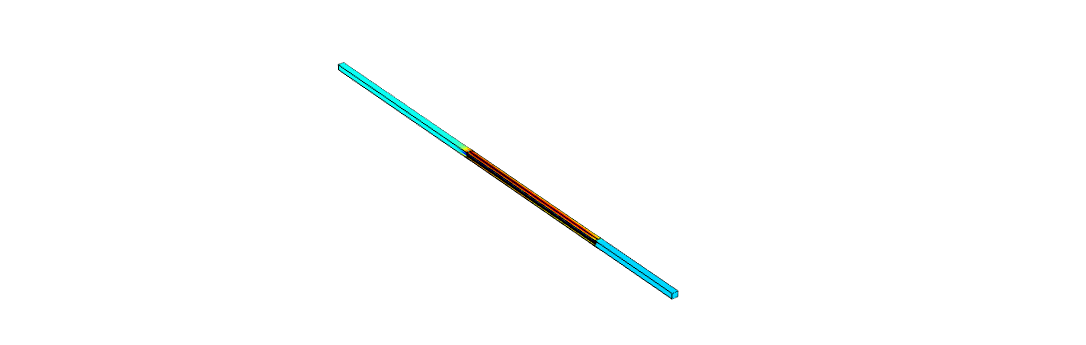
\includegraphics[width=0.8\textwidth]{00_Images/00_Velocity.png}
            \caption{Structure of a feedforward neural network.}
            \label{fig:neural_network}
        \end{figure}

        \subsection{Types of Layers}
        \noindent Neural networks have multiple types of layers, including:
            \begin{itemize}
                \item Input Layer: The first layer of the network that receives the input data.
                \item Hidden Layers: Intermediate layers that process the input data and extract features.
                \item Output Layer: The final layer that produces the output of the network.
            \end{itemize}
        \subsection{Shallow and Deep Neural Networks}
            \noindent Neural networks can be classified as shallow or deep based on the number of hidden layers they contain. Shallow networks have a small number of hidden layers, while deep networks have many hidden layers. Deep neural networks are capable of learning complex patterns and representations in the data but are more computationally intensive to train

    \section{Process of Supervised Learning}
        Supervised learning is a type of machine learning where the model is trained on labeled data. The objective is to learn a function that maps input data to the correct output based on the provided labels. The general process involves the following steps:

        \begin{enumerate}
            \item \textbf{Data Collection}: Gather a dataset consisting of input-output pairs. Let \( \mathbf{X} = \{ \mathbf{x}_1, \mathbf{x}_2, \ldots, \mathbf{x}_n \} \) be the set of input vectors and \( \mathbf{Y} = \{ y_1, y_2, \ldots, y_n \} \) be the corresponding set of output values.
            
            \item \textbf{Data Preprocessing}: Clean and preprocess the data to remove noise, handle missing values, and normalize the features. This step ensures that the data is in a suitable format for training the model.
            
            \item \textbf{Model Selection}: Choose a neural network architecture suitable for the problem. This includes deciding on the number of layers, the number of neurons per layer, and the type of activation functions.
            
            \item \textbf{Initialization}: Initialize the weights \( \mathbf{W} \) and biases \( \mathbf{b} \) of the network. This is typically done using small random values.
            
            \item \textbf{Forward Propagation}: Compute the predicted output \( \hat{y} \) by passing the input \( \mathbf{x} \) through the network.
            
            \item \textbf{Loss Computation}: Calculate the loss \( \mathcal{L}(\hat{y}, y) \) which measures the difference between the predicted output \( \hat{y} \) and the actual output \( y \).
            
            \item \textbf{Backward Propagation}: Compute the gradients of the loss with respect to the weights and biases.
            
            \item \textbf{Weight Update}: Update the weights and biases using an optimization algorithm such as Stochastic Gradient Descent (SGD).
            
            \item \textbf{Model Evaluation}: Evaluate the performance of the model on a validation set to tune hyperparameters and avoid overfitting.
        \end{enumerate}

        \noindent Mathematically, the process can be summarized as follows:

        \vspace{1em} \noindent Given an input vector \( \mathbf{x} \), the network's output \( \hat{y} \) is computed as:
        \begin{equation}
        \hat{y} = f(\mathbf{x}; \mathbf{W}, \mathbf{b})
        \end{equation}

        \noindent where \( f \) is the function represented by the neural network, parameterized by weights \( \mathbf{W} \) and biases \( \mathbf{b} \).

        \vspace{1em} \noindent The loss function \( \mathcal{L} \) is defined to measure the discrepancy between \( \hat{y} \) and the true output \( y \):
        \begin{equation}
        \mathcal{L}(\hat{y}, y)
        \end{equation}

        \vspace{1em} \noindent The gradients of the loss with respect to the parameters are computed during backpropagation:
        \begin{equation}
        \frac{\partial \mathcal{L}}{\partial \mathbf{W}}, \quad \frac{\partial \mathcal{L}}{\partial \mathbf{b}}
        \end{equation}

        \noindent Finally, the parameters are updated using an optimization algorithm:
        \begin{equation}
        \mathbf{W} \leftarrow \mathbf{W} - \eta \frac{\partial \mathcal{L}}{\partial \mathbf{W}}, \quad \mathbf{b} \leftarrow \mathbf{b} - \eta \frac{\partial \mathcal{L}}{\partial \mathbf{b}}
        \end{equation}

        \noindent where \( \eta \) is the learning rate.

    \begin{figure}[h]
        \centering
        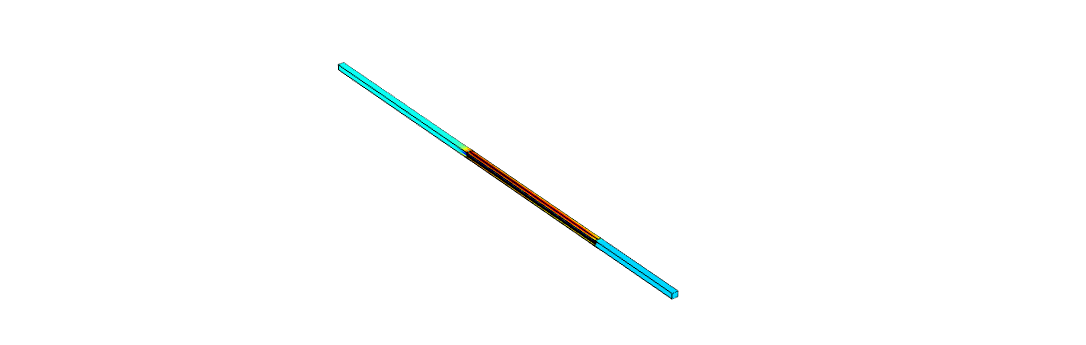
\includegraphics[width=0.8\textwidth]{00_Images/00_Velocity.png}
        \caption{Overview of the supervised learning process in neural networks.}
        \label{fig:supervised_learning}
    \end{figure}

    \section{Forward Propogation}
        Forward propagation is the process by which the input is passed through the neural network to obtain the output. It involves the computation of outputs at each layer of the network until the final output is achieved. The process can be described as follows:

        Given an input vector \( \mathbf{x} \), the output of the first layer is computed as:
        \begin{equation}
        \mathbf{z}^{(1)} = \mathbf{W}^{(1)} \mathbf{x} + \mathbf{b}^{(1)}
        \end{equation}
        \begin{equation}
        \mathbf{a}^{(1)} = \sigma(\mathbf{z}^{(1)})
        \end{equation}
        
        where \( \mathbf{W}^{(1)} \) and \( \mathbf{b}^{(1)} \) are the weights and biases of the first layer, \( \mathbf{z}^{(1)} \) is the linear combination of inputs and weights, and \( \sigma \) is the activation function.
        
        This process is repeated for each subsequent layer. For the \( l \)-th layer, the computations are:
        \begin{equation}
        \mathbf{z}^{(l)} = \mathbf{W}^{(l)} \mathbf{a}^{(l-1)} + \mathbf{b}^{(l)}
        \end{equation}
        \begin{equation}
        \mathbf{a}^{(l)} = \sigma(\mathbf{z}^{(l)})
        \end{equation}
        
        Finally, the output of the network is obtained:
        \begin{equation}
        \hat{y} = \mathbf{a}^{(L)}
        \end{equation}
        
        where \( L \) is the number of layers in the network.
        
        \begin{figure}[h]
            \centering
            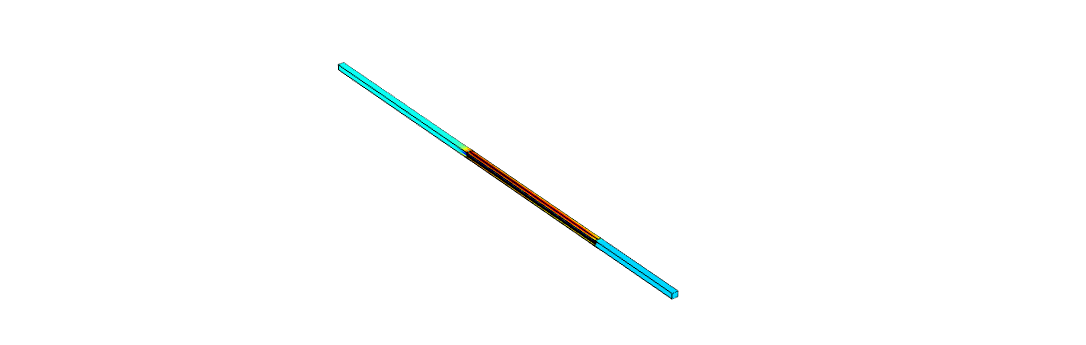
\includegraphics[width=0.8\textwidth]{00_Images/00_Velocity.png}
            \caption{Forward propagation through a neural network.}
            \label{fig:forward_propagation}
        \end{figure}
        
        \subsection{Activation Functions}
        
        Activation functions introduce non-linearity into the neural network, allowing it to learn complex patterns. Common activation functions include:
        
        \subsubsection{Sigmoid}
        
        The sigmoid function is defined as:
        \begin{equation}
        \sigma(z) = \frac{1}{1 + e^{-z}}
        \end{equation}
        It maps any real-valued number into the range (0, 1).
        
        \subsubsection{Hyperbolic Tangent (Tanh)}
        
        The tanh function is defined as:
        \begin{equation}
        \sigma(z) = \tanh(z) = \frac{e^z - e^{-z}}{e^z + e^{-z}}
        \end{equation}
        It maps any real-valued number into the range (-1, 1).
        
        \subsubsection{Rectified Linear Unit (ReLU)}
        
        The ReLU function is defined as:
        \begin{equation}
        \sigma(z) = \max(0, z)
        \end{equation}
        It outputs the input directly if it is positive; otherwise, it outputs zero.
        
        \subsubsection{Leaky ReLU}
        
        The Leaky ReLU function is defined as:
        \begin{equation}
        \sigma(z) = \begin{cases}
        z & \text{if } z \geq 0 \\
        \alpha z & \text{if } z < 0
        \end{cases}
        \end{equation}
        where \( \alpha \) is a small constant.
        
        \begin{figure}[h]
            \centering
            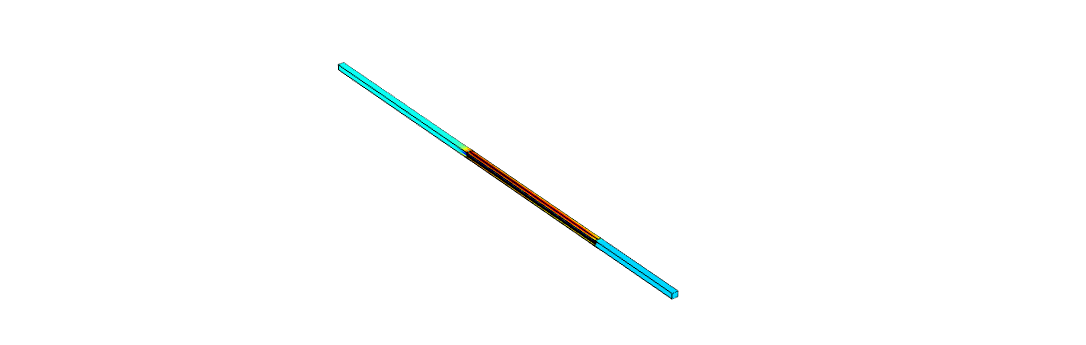
\includegraphics[width=0.8\textwidth]{00_Images/00_Velocity.png}
            \caption{Common activation functions used in neural networks.}
            \label{fig:activation_functions}
        \end{figure}
    
        \section{Backward Propagation}

            Backward propagation, or backpropagation, is the process by which neural networks update their weights and biases to minimize the loss function. It involves calculating the gradient of the loss function with respect to each weight by the chain rule, iterating backward from the output layer to the input layer. The main steps are as follows:
            
            \begin{enumerate}
                \item \textbf{Compute the loss}: Calculate the loss \( \mathcal{L} \) between the predicted output \( \hat{y} \) and the actual output \( y \).
                \item \textbf{Calculate the gradient of the loss with respect to the output layer}: For the output layer, compute the gradient of the loss with respect to the activations.
                \item \textbf{Propagate the gradient backward through the network}: Use the chain rule to compute the gradient of the loss with respect to the weights and biases of each layer.
                \item \textbf{Update the weights and biases}: Use the gradients to update the weights and biases in a direction that reduces the loss.
            \end{enumerate}
            
            Mathematically, the gradient of the loss \( \mathcal{L} \) with respect to the weights \( \mathbf{W}^{(l)} \) and biases \( \mathbf{b}^{(l)} \) in layer \( l \) is computed as:
            
            \begin{equation}
            \frac{\partial \mathcal{L}}{\partial \mathbf{W}^{(l)}} = \delta^{(l)} \mathbf{a}^{(l-1)} 
            \end{equation}
            
            \begin{equation}
            \frac{\partial \mathcal{L}}{\partial \mathbf{b}^{(l)}} = \delta^{(l)}
            \end{equation}
            
            where \( \delta^{(l)} \) is the error term for layer \( l \) and \( \mathbf{a}^{(l-1)} \) is the activation of the previous layer.
            
            The error term \( \delta^{(l)} \) is computed as:
            
            \begin{equation}
            \delta^{(l)} = \begin{cases} 
            (\mathbf{a}^{(L)} - y) \odot \sigma'(\mathbf{z}^{(L)}) & \text{for the output layer} \\
            (\mathbf{W}^{(l+1)})^T \delta^{(l+1)} \odot \sigma'(\mathbf{z}^{(l)}) & \text{for hidden layers}
            \end{cases}
            \end{equation}
            
            where \( \odot \) denotes the element-wise multiplication and \( \sigma' \) is the derivative of the activation function.
            
            \subsection{Loss Functions}
            
            Loss functions, also known as cost functions, measure how well the neural network's predictions match the actual target values. Common loss functions include:
            
            \subsubsection{Mean Squared Error (MSE)}
            
            The Mean Squared Error is used for regression tasks and is defined as:
            
            \begin{equation}
            \mathcal{L}_{\text{MSE}} = \frac{1}{n} \sum_{i=1}^n (\hat{y}_i - y_i)^2
            \end{equation}
            
            \begin{figure}[h]
                \centering
                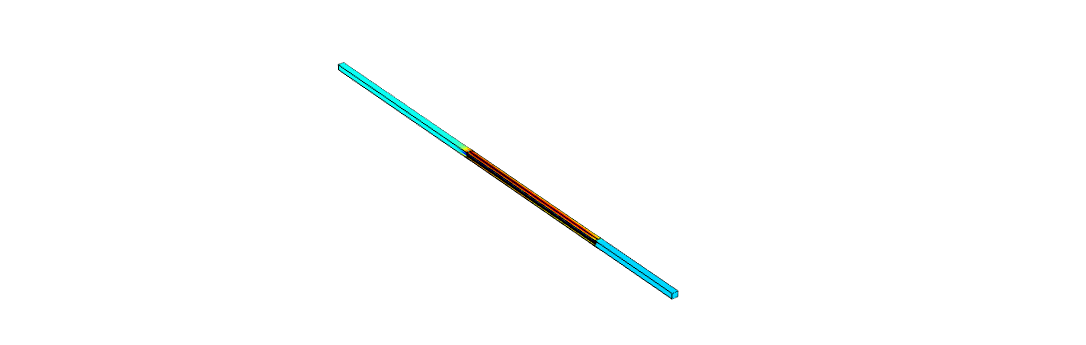
\includegraphics[width=0.8\textwidth]{00_Images/00_Velocity.png}
                \caption{Illustration of common loss functions.}
                \label{fig:loss_functions}
            \end{figure}
            
            \subsection{Methods to Update Weights}
            
            Updating the weights and biases of a neural network is a crucial part of the training process. Various methods can be employed to perform these updates:
            
            \subsubsection{Stochastic Gradient Descent (SGD)}
            
            SGD updates the weights using a single training example at a time:
            
            \begin{equation}
            \mathbf{W} \leftarrow \mathbf{W} - \eta \frac{\partial \mathcal{L}}{\partial \mathbf{W}}
            \end{equation}
            
            where \( \eta \) is the learning rate.
            
            \subsubsection{Batch Gradient Descent}
            
            Batch Gradient Descent computes the gradient using the entire training dataset:
            
            \begin{equation}
            \mathbf{W} \leftarrow \mathbf{W} - \eta \frac{1}{n} \sum_{i=1}^n \frac{\partial \mathcal{L}_i}{\partial \mathbf{W}}
            \end{equation}
            
            \subsubsection{Mini-Batch Gradient Descent}
            
            Mini-Batch Gradient Descent is a compromise between SGD and Batch Gradient Descent. It uses a small random subset (mini-batch) of the training data to compute the gradient:
            
            \begin{equation}
            \mathbf{W} \leftarrow \mathbf{W} - \eta \frac{1}{m} \sum_{i=1}^m \frac{\partial \mathcal{L}_i}{\partial \mathbf{W}}
            \end{equation}
            
            where \( m \) is the mini-batch size.
            
            \subsubsection{Adaptive Methods}
            
            Adaptive methods like AdaGrad, RMSProp, and Adam adjust the learning rate based on the history of the gradients. For example, the Adam optimization algorithm updates the weights as follows:
            
            \begin{equation}
            \mathbf{m}_t = \beta_1 \mathbf{m}_{t-1} + (1 - \beta_1) \frac{\partial \mathcal{L}}{\partial \mathbf{W}}
            \end{equation}
            
            \begin{equation}
            \mathbf{v}_t = \beta_2 \mathbf{v}_{t-1} + (1 - \beta_2) \left( \frac{\partial \mathcal{L}}{\partial \mathbf{W}} \right)^2
            \end{equation}
            
            \begin{equation}
            \hat{\mathbf{m}}_t = \frac{\mathbf{m}_t}{1 - \beta_1^t}
            \end{equation}
            
            \begin{equation}
            \hat{\mathbf{v}}_t = \frac{\mathbf{v}_t}{1 - \beta_2^t}
            \end{equation}
            
            \begin{equation}
            \mathbf{W} \leftarrow \mathbf{W} - \eta \frac{\hat{\mathbf{m}}_t}{\sqrt{\hat{\mathbf{v}}_t} + \epsilon}
            \end{equation}
            
            where \( \beta_1 \) and \( \beta_2 \) are hyperparameters, \( \mathbf{m}_t \) and \( \mathbf{v}_t \) are the first and second moment estimates, and \( \epsilon \) is a small constant.
            
            \begin{figure}[h]
                \centering
                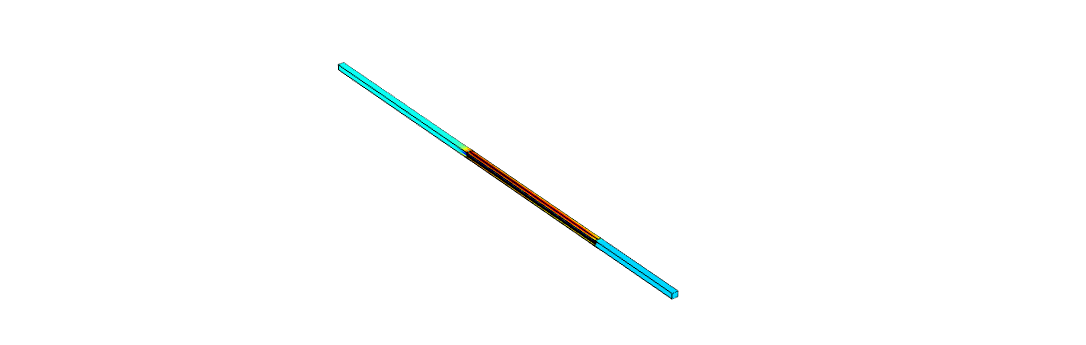
\includegraphics[width=0.8\textwidth]{00_Images/00_Velocity.png}
                \caption{Comparison of different methods to update weights.}
                \label{fig:update_methods}
            \end{figure}

    \section{Hyperparameters}

        Hyperparameters are parameters whose values are set before the learning process begins. Unlike model parameters, which are learned during training, hyperparameters control the training process and influence the performance of the neural network. Common hyperparameters include learning rate, batch size, number of epochs, network architecture, activation functions, weight initialization, dropout rate, and regularization parameters.
        
        \subsection{Common Hyperparameters}
        
        \subsubsection{Learning Rate}
        
        The learning rate \( \eta \) controls the size of the steps taken during gradient descent to update the weights. A smaller learning rate can lead to more precise convergence but slower training, while a larger learning rate can speed up training but might overshoot the optimal solution.
        
        \subsubsection{Batch Size}
        
        Batch size determines the number of training examples used to calculate the gradient in one forward/backward pass. It influences the stability and speed of the training process. Common choices are small (stochastic gradient descent), large (batch gradient descent), or in between (mini-batch gradient descent).
        
        \subsubsection{Number of Epochs}
        
        The number of epochs defines how many times the entire training dataset passes through the network. More epochs typically improve learning, but excessive epochs can lead to overfitting.
        
        \subsubsection{Network Architecture}
        
        Network architecture includes the number of layers, the number of neurons per layer, and the type of layers used (e.g., dense, convolutional, recurrent). These choices significantly impact the capacity and capability of the network.
        
        \subsubsection{Activation Functions}
        
        Different activation functions (e.g., Sigmoid, Tanh, ReLU) can be used in different layers of the network. The choice of activation function affects the network's ability to capture non-linear patterns.
        
        \subsubsection{Weight Initialization}
        
        Weight initialization affects the starting point of the training process. Common initialization methods include random initialization, Xavier initialization, and He initialization, each suitable for different types of activation functions.
        
        \subsubsection{Dropout Rate}
        
        Dropout is a regularization technique where a fraction of neurons is randomly set to zero during training. The dropout rate controls this fraction and helps prevent overfitting by promoting the independence of neurons.
        
        \subsubsection{Regularization Parameters}
        
        Regularization parameters, such as L1 and L2 regularization, add a penalty to the loss function to constrain the model complexity. They help in preventing overfitting by discouraging overly complex models.
        
        \begin{figure}[h]
            \centering
            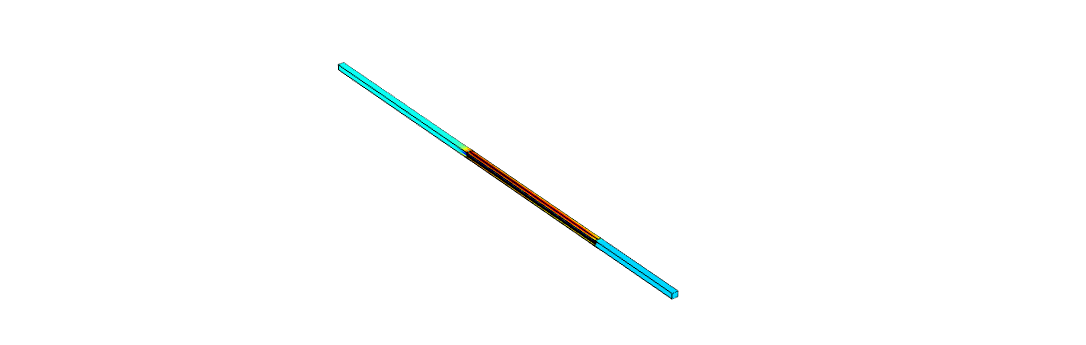
\includegraphics[width=0.8\textwidth]{00_Images/00_Velocity.png}
            \caption{Overview of common hyperparameters in neural networks.}
            \label{fig:hyperparameters}
        \end{figure}
        
        \subsection{Hyperparameter Optimization}
        
        Hyperparameter optimization involves finding the optimal set of hyperparameters that result in the best performance of the neural network. Common methods for hyperparameter optimization include:
        
        \subsubsection{Grid Search}
        
        Grid search involves specifying a set of values for each hyperparameter and training the model on all possible combinations of these values. It is computationally expensive but exhaustive.
        
        \begin{equation}
        \text{Optimal Hyperparameters} = \arg \min_{\eta, \text{batch size}, \ldots} \text{Validation Loss}
        \end{equation}
        
        \subsubsection{Random Search}
        
        Random search samples random combinations of hyperparameters from a predefined distribution. It is often more efficient than grid search and can find good hyperparameters with fewer iterations.
        
        \begin{equation}
        \text{Optimal Hyperparameters} = \arg \min_{\eta, \text{batch size}, \ldots} \text{Validation Loss}
        \end{equation}
        
        \subsubsection{Bayesian Optimization}
        
        Bayesian optimization builds a probabilistic model of the objective function and uses it to select the most promising hyperparameters to evaluate next. It is more sophisticated and can find optimal hyperparameters more efficiently.
        
        \begin{equation}
        \text{Optimal Hyperparameters} = \arg \max_{\eta, \text{batch size}, \ldots} P(\text{Low Validation Loss} \mid \eta, \text{batch size}, \ldots)
        \end{equation}
        
        \subsubsection{Hyperband}
        
        Hyperband is a method that combines random search with early stopping. It evaluates many configurations with a small number of iterations and progressively increases the budget for the most promising configurations.
        
        \begin{equation}
        \text{Optimal Hyperparameters} = \arg \min_{\eta, \text{batch size}, \ldots} \text{Validation Loss}
        \end{equation}
        
        \begin{figure}[h]
            \centering
            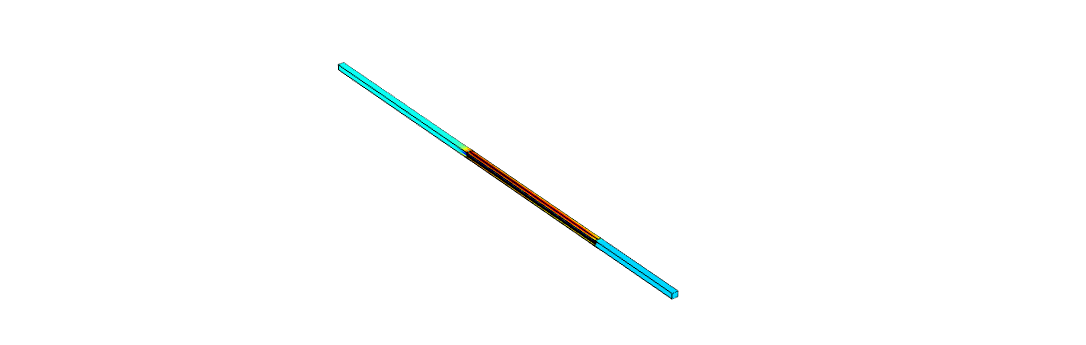
\includegraphics[width=0.8\textwidth]{00_Images/00_Velocity.png}
            \caption{Comparison of different hyperparameter optimization methods.}
            \label{fig:hyperparameter_optimization}
        \end{figure}
    
\newpage \chapter{Literature Review}

\newpage \chapter{Materials and Methods}

    % Define custom column types with different proportional widths
    \newcolumntype{D}{>{\hsize=0.5\hsize}X} % Adjust these ratios as needed
    \newcolumntype{E}{>{\hsize=0.5\hsize}X}
    \newcolumntype{F}{>{\hsize=2.5\hsize}X}
    \newcolumntype{G}{>{\hsize=0.5\hsize}X}

    \newpage \begin{table}[H]
    \centering
    \begin{tabularx}{\textwidth}{DEFG} % Custom column widths
    \toprule
    \textbf{Header} & \textbf{Symbol} & \textbf{Explanation} & \textbf{Unit} \\ 
    \midrule
    \multicolumn{4}{c}{\textbf{Input Parameters}} \\
    \midrule
    Q & \( Q \) & \textbf{Heat generation} influences membrane hydration and operational efficiency; critical to prevent membrane dry-out and maintain ion conductivity. & \( \text{Wm}^{-2} \) \\
    Tamb & \( T_{amb} \) & \textbf{Ambient temperature of the air} sets baseline thermal conditions; higher temperatures boost performance to a limit before causing potential overheating. & \( \degree C \) \\
    Uin & \( U_{in} \) & \textbf{Airflow velocity} determines oxygen supply rate, essential for maintaining optimal reaction rates and power output. & \( \text{m/s} \) \\
    Wcc & \( W_{cc} \) & \textbf{Cathode channel width} determines oxygen flow and diffusion rates to the cathode, crucial for optimizing reaction efficiency. & \( \text{mm} \) \\
    Hcc & \( H_{cc} \) & \textbf{Cathode channel height} affects gas flow resistance and water removal, essential for maintaining membrane hydration and preventing flooding. & \( \text{mm} \) \\
    Lcc & \( L_{cc} \) & \textbf{Cathode channel length} influences the residence time of reactants and products along the channel, impacting overall fuel cell efficiency. & \( \text{mm} \) \\ 
    Wr & \( W_{r} \) & \textbf{Rib width} supports mechanical stability and maximizes the active area available for reactions, balancing structural support with performance. & \( \text{mm} \) \\
    Hr & \( H_{r} \) & \textbf{Rib height} controls the depth of flow channels, enhancing reactant distribution and efficient water management within the stack. & \( \text{mm} \) \\
    \midrule
    \multicolumn{4}{c}{\textbf{Output Performance Metrics}} \\
    \midrule
    Tsta & \( T_{stack} \) & \textbf{Stack temperature} is crucial for optimal reaction rates, membrane hydration, and to prolong the lifespan. & \( \degree C \) \\ 
    Delp & \( \Delta p \) & \textbf{Pressure drop} indicates the system's resistance to reactant flow; minimizing pressure drop is essential to enhance efficiency and ensure uniform distribution. & \( \text{Pa} \) \\ 
    \bottomrule
    \end{tabularx}
    \caption{Detailed Explanation of Variables}
    \end{table}
    
\chapter{COMSOL Model}
    \section{Model Assumptions}
        \begin{enumerate}
            \item The airflow entering the channel is turbulent. The Reynolds number exceeds 2300 at an inlet velocity ($U_{in}$) of 0.3 m/s.
            \item Portions of the fuel cell not part of the cathode flow field are impermeable to air. While carbon paper is porous, the in-plane pressure drop is much greater than that of the cathode flow field.
            \item The cathode flow field channels are modeled with a uniform height. The average offset (0.025 mm) is negligible compared to the channel height (1 mm).
            \item Cathode flow fields are modeled with straight edges and right-angle folds. The fold radius (0.05 mm) is small compared to the channel width (1 mm).
            \item Conservation of mass and momentum of airflow is assumed to be valid when transitioning between open spaces and cathode channels.
            \item A representative unit cell approximates the entire stack, excluding edge effects near the terminals. Airflow entering the unit cell is uniform and symmetrical.
            \item Channels are identical throughout the stack, resulting in no pressure drop differences between channels.
            \item The channels are fully dry without condensation. The oxidant stoichiometry exceeds 100, ensuring water vapor produced is absorbed by the airflow, negating the need for accounting water saturation.
            \item The losses from the fuel cell operation are converted to heat. 
        \end{enumerate}

        \section{Workflow - Pressure Drop}
        The following steps outline the workflow process for the unit cell simulations conducted in COMSOL:

        \begin{enumerate}
            \item \textbf{Selection of Laminar Flow Model:}
            \begin{itemize}
                \item This model was chosen because the airflow within the channels is laminar and is the largest contributor to the pressure drop across the stack.
                \item The laminar flow model allows for faster convergence and has been shown to be accurate when compared with experimental results.
            \end{itemize}
            
            \item \textbf{Construction of Unit Cell:}
            \begin{itemize}
                \item The unit cell was constructed using blocks with dimensions defined by equations to accommodate dimensional changes in the channels.
            \end{itemize}
            
            \item \textbf{Meshing Strategy:}
            \begin{itemize}
                \item A custom mesh was employed, focusing on the transition areas between inflow and outflow within the channels with a finer mesh.
                \item A coarser mesh was used within the channel and the air space between inflow and outflow.
                \item A mesh independence study was performed during the mesh fine-tuning. The results are shown in Figure ?.
                \item The difference between the blue dash (custom meshing) and green dots (physics-based extra fine meshing) is less than 3\%, thus the blue dash mesh was selected for its speed and accuracy.
            \end{itemize}
            
            \item \textbf{Parameter Sweep Function:}
            \begin{itemize}
                \item The parameter sweep function was utilized to explore all possible combinations for each stack size.
            \end{itemize}
            
            \item \textbf{Exporting Simulation Data:}
            \begin{itemize}
                \item The inputs and outputs of the simulations were exported from COMSOL for further analysis.
            \end{itemize}
        \end{enumerate}

        \section{Workflow - Temperature Stack}
        The following steps outline the workflow process for the unit cell simulations conducted in COMSOL:

        \begin{enumerate}
            \item \textbf{Selection of Physics Models:}
            \begin{itemize}
                \item The unit cell simulations were done using laminar flow physics as well as heat transfer in laminar flow.
                \item The parameter sweep function was utilized to explore all possible combinations in the parameter space.
                \item This model was selected because the flow through the channel is laminar and the simulation focuses on heat transfer within the channels.
            \end{itemize}
            
            \item \textbf{Construction of Unit Cell:}
            \begin{itemize}
                \item The unit cell was constructed using blocks with dimensions defined by equations to accommodate dimensional changes in the channels.
            \end{itemize}
            
            \item \textbf{Heat Generation Simulation:}
            \begin{itemize}
                \item Heat generation was simulated as a boundary heat source placed at the cathode side of the membrane.
            \end{itemize}
            
            \item \textbf{Heat Conduction Values:}
            \begin{itemize}
                \item The heat conduction values for each layer in the fuel cell were obtained from various papers, as shown in Table 8-1.
            \end{itemize}
            
            \item \textbf{Meshing Strategy:}
            \begin{itemize}
                \item A mesh independence study was conducted during the fine-tuning of the mesh. The results are shown in Figure ?.
                \item The difference between the blue dash and green dots is less than 1.06\%, hence the blue dash mesh was selected for its speed and accuracy.
            \end{itemize}
            
            \item \textbf{Exporting Simulation Data:}
            \begin{itemize}
                \item The inputs and outputs of the simulations were exported from COMSOL for further analysis.
            \end{itemize}
        \end{enumerate}

    \newpage \section{Parameters}
    
        \begin{table}[h]
        \centering
        \begin{tabularx}{\textwidth}{X X X}
        \toprule
        \textbf{Name} & \textbf{Value} & \textbf{Unit} \\ 
        \midrule
        Cell Area & 0.005 & m$^2$ \\ 
        Cell Voltage & 0.6 & V \\ 
        Compression & 0.1 & - \\ 
        Current & 40 & A \\ 
        Hbp & 5$\times$10$^{-5}$ & m \\ 
        Hcc & 1.25$\times$10$^{-3}$ & m \\ 
        Hcp & 3.15$\times$10$^{-4}$ & m \\ 
        Hmem & 1.5$\times$10$^{-5}$ & m \\ 
        Kcp & 1.5 & W$\cdot$m$^{-1}$K$^{-1}$ \\ 
        Kmem & 0.1 & W$\cdot$m$^{-1}$K$^{-1}$ \\ 
        Lcc & 0.03 & m \\ 
        pRef & 1.0133$\times$10$^5$ & Pa \\ 
        Q & 5040 & W$\cdot$m$^{-2}$ \\ 
        Tamb & 293.15 & K \\ 
        Test & 25.2 & W \\ 
        Uin & 7.75 & m$\cdot$s$^{-1}$ \\ 
        Wcc & 0.001 & m \\ 
        Wr & 5$\times$10$^{-5}$ & m \\ 
        \bottomrule
        \end{tabularx}
        \caption{Parameter Values}
        \label{tab:parameters}
        \end{table}
    
    \section{Materials}
        % Superscripts Table
        \begin{table}[H]
        \centering
        \begin{tabularx}{\textwidth}{BA}
        \toprule
        \textbf{Name} & \textbf{Unit} \\ 
        \midrule
        \multicolumn{2}{c}{\textbf{Air}} \\
        \midrule
        Dynamic viscosity & \( \text{Pa} \cdot \text{s} \) \\ 
        Ratio of specific heats & - \\ 
        Heat capacity at constant pressure & \(\text{J} / (\text{kg} \cdot \text{K})\) \\ 
        Density & \(\text{kg} / \text{m}^{3}\) \\ 
        Thermal conductivity & \(\text{W} / (\text{m} \cdot \text{K})\) \\
        \midrule
        \multicolumn{2}{c}{\textbf{Carbon Paper}} \\
        Density & \(\text{kg} / \text{m}^{3}\) \\ % No value
        Heat capacity at constant pressure & \(\text{J} / (\text{kg} \cdot \text{K})\) \\ % No value
        Thermal conductivity & \(\text{W} / (\text{m} \cdot \text{K})\) \\
        \midrule
        \midrule
        \multicolumn{2}{c}{\textbf{Membrane}} \\
        Thermal conductivity & \(\text{W} / (\text{m} \cdot \text{K})\) \\
        \midrule
        \midrule
        \multicolumn{2}{c}{\textbf{Steel Grade 316L}} \\
        Density & \(\text{kg} / \text{m}^{3}\) \\ % No value
        Heat capacity at constant pressure & \(\text{J} / (\text{kg} \cdot \text{K})\) \\ % No value
        Thermal conductivity & \(\text{W} / (\text{m} \cdot \text{K})\) \\
        \midrule
        \bottomrule
        \end{tabularx}
        \caption{Material Descriptions}
        \end{table}

    
    \section{Laminar Flow}
        \subsection{Governing Equations}
            \begin{equation}
                \rho (\textbf{u} \cdot \nabla) \textbf{u} = \nabla \cdot \left[-p\textbf{I} + \textbf{K} \right] + \textbf{F} 
            \end{equation}
                \noindent where \(\rho\) is the density of air, \textbf{u} is the velocity vector, p is the pressure, \textbf{I} is the identity matrix, \textbf{K} is the viscous stress tensor, and \textbf{F} is the volume force vector.
            \begin{equation}
                \nabla \cdot (\rho \textbf{u})= 0 % The equation is different in the thesis
            \end{equation}
            \begin{equation}
                \textbf{K} = \mu (\nabla \textbf{u} + (\nabla \textbf{u})^T) - \frac{2}{3} \mu (\nabla \cdot \textbf{u})\textbf{I} % NOTE: The equation is different from the one in the thesis.
            \end{equation}
                where \textbf{\(\mu\)} is the dynamic viscosity of air. 
    
        \subsection{Initial Values}
            \begin{enumerate}
                \item Velocity field
                    \begin{equation}
                        \textbf{u} = \textbf{0}
                    \end{equation}
                \item Pressure
                    \begin{equation}
                        p = 0
                    \end{equation}
            \end{enumerate}

        \subsection{Boundary Conditions}
            \begin{enumerate}
                \item Wall (No slip)
                    \begin{equation}
                        \mathbf{u} = \mathbf{0}
                    \end{equation}
            
                \item Inlet (Velocity)
                    \begin{equation}
                        \mathbf{u} = -U_{0} \mathbf{n}
                    \end{equation}
                        where \(U_{0}\) is the initial velocity (i.e. normal inflow velocity) and \(\mathbf{n}\) is the unit normal vector. 
                
                \item Outlet (Pressure)
                    \begin{equation}
                        \left[-p\textbf{I} + \textbf{K} \right]\mathbf{n} = - \hat{p}_{0} \mathbf{n} % this equation is different from the one in the thesis.
                    \end{equation}
                    \begin{equation}
                        \hat{p_{0}} \leq p_{0}, \nabla \mathbf{G} \cdot \mathbf{n} = 0
                    \end{equation}
                        where \(\hat{p}_{0}\) is the estimated standard condition pressure, \(p_{0}=0\) is the standard condition pressure (i.e. suppress backflow), \(\mathbf{G}\) is the reciprocal wall distance. 
            
                \item Symmetry 
                    \begin{equation}
                        \mathbf{u} \cdot \mathbf{n} = 0
                    \end{equation}
                    \begin{equation}
                        \mathbf{K}_{n} - (\mathbf{K}_{n} \cdot \mathbf{n})\mathbf{n} = 0, \mathbf{K}_{n} = \mathbf{Kn}
                    \end{equation}
            \end{enumerate}
            
    \section{Heat Transfer}
        \subsection{Governing Equations - Solid}
            \begin{equation}
                \rho C_{p} \textbf{u} \cdot \nabla T + \nabla \cdot \textbf{q} = Q + Q_{ted}
            \end{equation}
                \noindent where \(C_{p}\) is the specific heat capacity of air, T is the temperature of air, \textbf{q} is the heat flux vector, Q is the heat source, and \(Q_{ted}\) is the thermoelastic damping heat source.
            \begin{equation}
                \textbf{q} = -k \nabla T
            \end{equation}
                \noindent where k is the thermal conductivity. 
            \begin{equation}
                Q = (1.23 - Operating\ Voltage) \times \frac{Fuel\ Cell\ Stack\ Current}{Cell\ Area}
            \end{equation}
                
        \subsection{Governing Equations - Fluid}
            \begin{equation}
                \rho C_{p} \textbf{u} \cdot \nabla T + \nabla \cdot \textbf{q} = Q + Q_{p} + Q_{vd} % I dont know what vd is.
            \end{equation}
            \noindent where \(Q_{p}\) is the point heat source.
            \begin{equation}
                \textbf{q} = -k \nabla T
            \end{equation}
        
        \subsection{Governing Equations - Thin Layer}
            \begin{equation}
                -\textbf{n}_{d} \cdot \textbf{q}_{u} = \frac{(T_{u} - T_{d})}{R_{s}} + \frac{1}{2} d_{s} Q_{s}
            \end{equation}
            \noindent where \(R_s\) is the thermal resistance, and \(d_s\) is the thin layer thickness. 
            \begin{equation}
                -\textbf{n}_{u} \cdot \textbf{q}_{u} = \frac{(T_{d} - T_{u})}{R_{s}} + \frac{1}{2} d_{s} Q_{s}
            \end{equation}
            \begin{equation}
                R_{s} = \frac{d_{s}}{k_{s}}
            \end{equation}
        
        \subsection{Initial Values}
            \begin{enumerate}
                \item Temperature
                    \begin{equation}
                        T = T_{amb}
                    \end{equation}
                    where \(T_{amb}\) is the initial ambient temperature.
            \end{enumerate}
    
        \subsection{Boundary Conditions}
            \begin{enumerate}
                \item Insulation
                    \begin{equation}
                        -\mathbf{n} \cdot \mathbf{q} = 0
                    \end{equation}
            
                \item Symmetry
                    \begin{equation}
                        -\mathbf{n} \cdot \mathbf{q} = 0
                    \end{equation}
            
                \item Boundary Heat Source
                    \begin{equation}
                        -\mathbf{n} \cdot \mathbf{q} = Q_b
                    \end{equation}
                    where \(Q_b\) is the boundary heat source.
                
                \item Outflow
                    \begin{equation}
                        -\mathbf{n} \cdot \mathbf{q} = 0
                    \end{equation}
            
                \item Inlet
                    \begin{equation}
                        T = T_{amb}
                    \end{equation}
            \end{enumerate}
    
    \section{Mesh}
    
    \section{Study}
        \subsection{Difference between External and Internal Sweep}
            An internal sweep involves varying parameters directly within the 
            simulation model itself. This type of sweep is integrated into the 
            simulation process, where the solver automatically adjusts the parameters 
            as part of its internal algorithm. Internal sweeps are typically used to 
            explore the parameter space of the model in a more automated and 
            controlled manner, often leveraging the solver's built-in capabilities 
            to iterate through different parameter values.

            
            \vspace{1em} \noindent An external sweep, on the other hand, involves varying parameters outside 
            of the simulation model. This is usually managed by an external script 
            or control mechanism that systematically modifies the input parameters, 
            runs the simulation for each set of parameters, and collects the results. 
            External sweeps provide more flexibility and control over the parameter 
            variations and can be useful for complex scenarios where the internal 
            capabilities of the solver might be limited.
        \subsection{Parametric Sweep}
            A parametric sweep is a systematic method used in simulations and computational 
            experiments to explore the effects of varying parameters within a defined range. 
            By adjusting one or more input parameters incrementally, researchers can observe 
            how changes influence the outcome, enabling a comprehensive analysis of the 
            system's behavior. This technique is essential for optimizing designs, 
            identifying critical factors, and understanding the sensitivity of the results 
            to different variables. Ultimately, parametric sweeps provide valuable insights 
            that drive informed decision-making and innovation.

            \begin{table}[h]
            \centering
            \begin{tabularx}{\textwidth}{X X X}
            \toprule
            \textbf{Name} & \textbf{Values} & \textbf{Unit} \\ 
            \midrule
            Hcc & 1 1.25 1.5 1.75 2 & \(\text{mm}\) \\ 
            Wcc & 0.5 0.75 1 1.25 1.5 & \(\text{mm}\) \\ 
            Lcc & 30 60 90 & \(\text{mm}\) \\ 
            \bottomrule
            \end{tabularx}
            \caption{Parameter Sweep Values for All Combinations}
            \end{table}
        \subsection{Auxilary Sweep}
            An auxiliary sweep is a computational technique used to study the influence
            of secondary parameters or variables that are not directly part of the main 
            parametric study. It involves varying these auxiliary parameters to 
            investigate their impact on the primary simulation or experiment results. 
            This approach helps in understanding the interactions and dependencies 
            between primary and auxiliary parameters, providing a deeper insight into 
            the system's overall behavior. Auxiliary sweeps are particularly useful in 
            complex models where multiple factors may indirectly affect the outcomes, 
            aiding in fine-tuning and enhancing the accuracy of simulations.

            \begin{table}[h]
            \centering
            \begin{tabularx}{\textwidth}{X X X}
            \toprule
            \textbf{Name} & \textbf{Values} & \textbf{Unit} \\ 
            \midrule
            Uin & 1 3.25 5.5 7.75 10 & \(\text{m}/\text{s}\) \\ 
            Q & 1272 3132 5040 & \(W/\text{m}^{-2}\) \\ 
            Tamb & -20 0 20 40 & \(\degree \text{C}\) \\ 
            \bottomrule
            \end{tabularx}
            \caption{Auxilary Sweep Values for All Combinations}
            \end{table}
        
        \section{Results}
            \subsection{Accumulated Probe Table: Set 1}
                \begin{enumerate}
                    \item Hcc (1 - hc)
                    \item Wcc (2 - wc)
                    \item Lcc (3 - length)
                    \item Tamb (4 - Tamb)
                    \item Q (5 - Q)
                    \item Uin (6 - Uin)
                    \item Delp (15 - Pressure (Pa), Pressure Probe 3)
                        \begin{figure}[H]
                            \centering
                            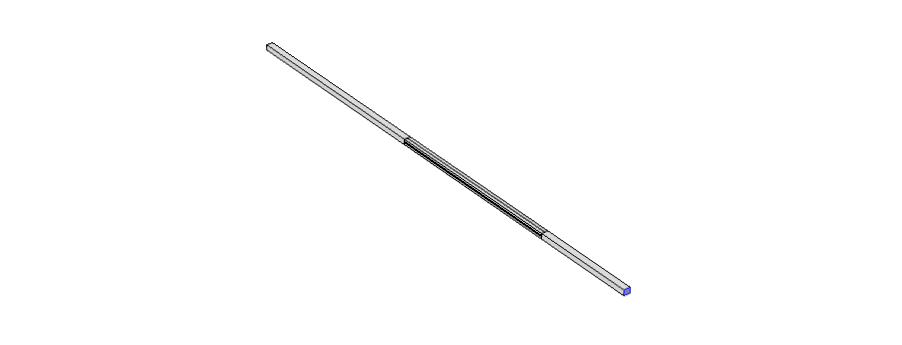
\includegraphics[width=0.75\textwidth]{00_Images/00_Pressure_Probe_3.png}
                            \caption{Pressure Probe 3 Location}
                        \end{figure}
                    \item Tsta (18 - Temperature (degC), Stack Temperature Probe 1)
                        \begin{figure}[H]
                            \centering
                            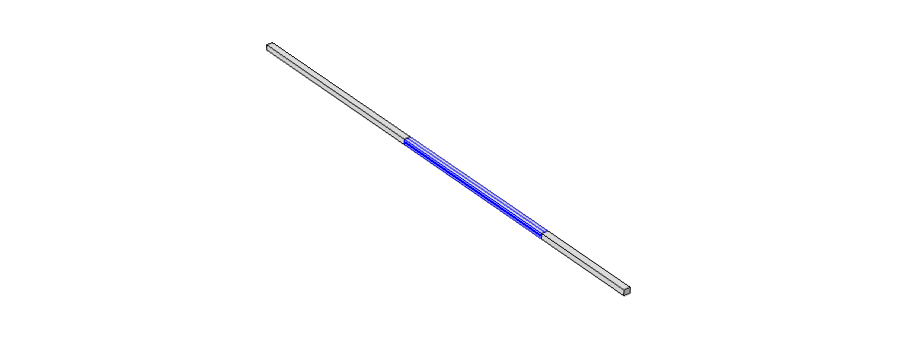
\includegraphics[width=0.75\textwidth]{00_Images/00_Stack_Temperature_Probe_1.png}
                            \caption{Stack Temperature Probe 1 Location}
                        \end{figure}
                \end{enumerate}

            \subsection{3D Plots}
                \begin{enumerate}
                    \item Pressure Drop
                        \begin{figure}[H]
                            \centering
                            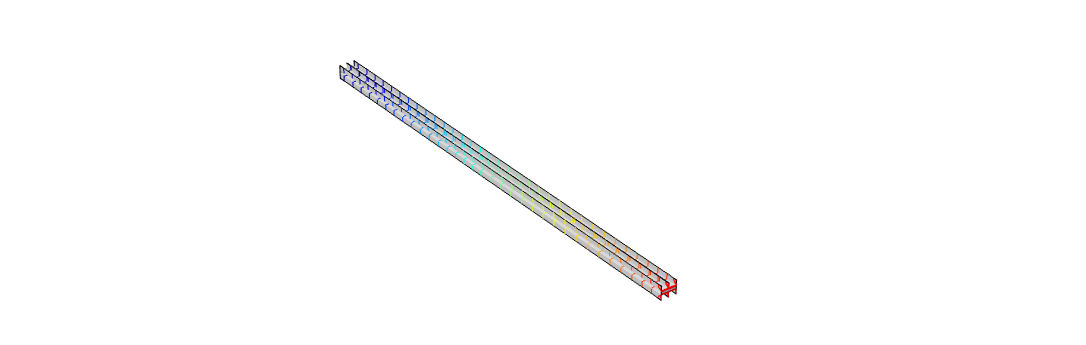
\includegraphics[width=0.75\textwidth]{00_Images/00_Pressure.png}
                            \caption{Pressure Drop 3D Plot}
                        \end{figure}
                    \item Temperature Stack
                        \begin{figure}[H]
                            \centering
                            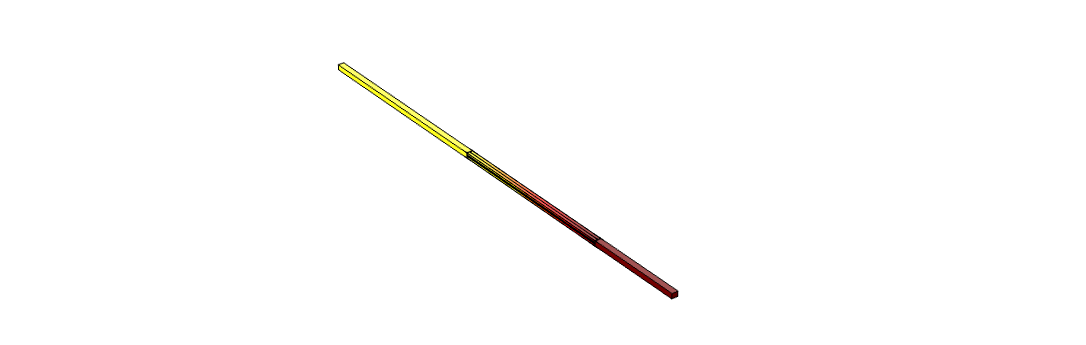
\includegraphics[width=0.75\textwidth]{00_Images/00_Temperature.png}
                            \caption{Temperature Stack 3D Plot}
                        \end{figure}
                    \item Velocity 
                        \begin{figure}
                            \centering
                            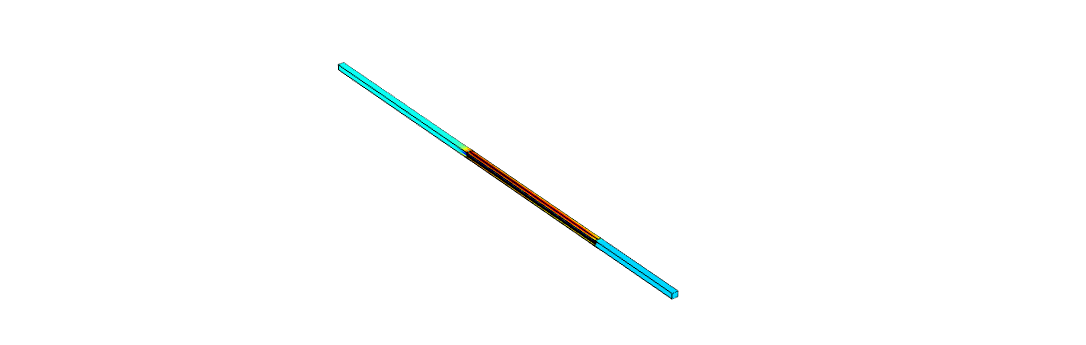
\includegraphics[width=0.75\textwidth]{00_Images/00_Velocity.png}
                            \caption{Velocity 3D Plot}
                        \end{figure}
                \end{enumerate}





\section{Conclusion}
\section{Outlook}
\section{References}

\end{document}
